\documentclass[aspectratio=169]{beamer}

% ===================================================================
% THEME AND APPEARANCE
% ===================================================================
\usetheme{Madrid}
\usecolortheme{seahorse}
\setbeamertemplate{navigation symbols}{}
\setbeamertemplate{footline}[frame number]
\setbeamertemplate{blocks}[rounded][shadow=false]

% ===================================================================
% PACKAGES
% ===================================================================
% Encoding & fonts
\usepackage[T1]{fontenc}
\usepackage[utf8]{inputenc}

% Math and Algorithms
\usepackage{amsmath,amssymb}
\usepackage{algorithm}
\usepackage{algpseudocode} % For the paper-style algorithm formatting

% Graphics and Diagrams
\usepackage{tikz}
\usetikzlibrary{calc, arrows.meta, positioning, shapes.geometric, shapes.misc, fit}
\usepackage{adjustbox} % NEW: For better scaling of figures and boxes to prevent overflows

% Other utilities
\usepackage{qrcode} % For the final artifact QR code
\usepackage{xcolor} % NEW: Explicitly load for color definitions (though Beamer implies it)

% ===================================================================
% CUSTOM COLORS AND COMMANDS
% ===================================================================
% Define the consistent color scheme from your paper/previous slides
\definecolor{pivotblue}{RGB}{32,102,170}
\definecolor{updategreen}{RGB}{56,142,60}
\definecolor{depred}{RGB}{198,40,40}
\definecolor{accent}{RGB}{123,31,162}
\definecolor{darkgreen}{rgb}{0,0.5,0}
% A custom environment for compact bullet points if needed later
\newenvironment{tightitem}{%
  \begin{itemize}\setlength{\itemsep}{2pt}\setlength{\parskip}{0pt}
}{\end{itemize}}

% NEW: Custom command for consistent figure captions
\newcommand{\figcap}[1]{\vspace{1mm}{\scriptsize \emph{#1}}}
% Add these lines to the package section of main.tex

\usepackage{pgfplots}
\pgfplotsset{compat=1.17} % Or your installed version
% ===================================================================
% PRESENTATION METADATA
% ===================================================================
\title[Parallel QR for SLSQP]{Efficient Task-Graph Scheduling for Parallel QR Factorization in SLSQP}
\author{Soumyajit Chatterjee, Rahul Utkoor, Uppu Eshwar, Sathya Peri, V.K. Nandivada}
\institute[IITH, Qualcomm, IITM]{Indian Institute of Technology, Hyderabad \\ QUALCOMM India Private Limited \\ Indian Institute of Technology, Madras}
\date{Euro-Par 2025} % CHANGED: Updated to match paper's implied year (2025, per artifact DOI)

% ===================================================================
% DOCUMENT BODY
% ===================================================================
\begin{document}

	% --- The Title Page ---
	\begin{frame}
	  \titlepage
	\end{frame}
	
	% --- The Presentation Slides (Following Your New Flow) ---
	% Note: You will need to create these .tex files as we proceed.
	% I am using descriptive filenames based on our new plan.
	
	\begin{frame}{Agenda}
	\pause 	
	\begin{block}{Talk Roadmap}
		\begin{enumerate}\setlength{\itemsep}{6pt}
		  \item Motivation: Optimization in Practice
		  \item Why Focus on QR Factorization?
		  \item The Sequential QR Algorithm
		  \item A Naive Approach: Parallelism with Barriers
		  \item Problem Formulation: QR as a Task DAG
		  \item Research Question and Contributions
		  \item Our Solution: Asynchronous Two-Queue Scheduling
		\end{enumerate}
	\end{block}
\end{frame}
	\begin{frame}{Motivation: Optimization in Practice}
	\pause 
	\begin{columns}[c,onlytextwidth]
		\column{0.60\textwidth}
		\begin{block}{Context}
		  \begin{itemize}\setlength{\itemsep}{4pt}
		    \item Many applications in \textbf{ML, robotics, and scientific computing} rely on nonlinear optimization.
		    \item \textbf{NLopt} is a widely used library providing optimization algorithms.
		    \item Among them, \textbf{SLSQP} (Sequential Least Squares Quadratic Programming) is popular for constrained problems.
		  \end{itemize}
		\end{block}
	
		\column{0.40\textwidth}
		\centering
		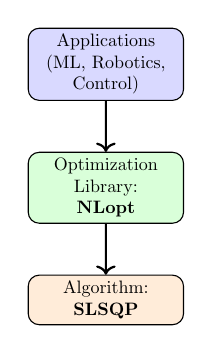
\begin{tikzpicture}[node distance=1cm and 0.8cm, scale=0.65, transform shape]
		  \node[draw, rounded corners, fill=blue!15, text width=2.8cm, align=center] (apps) {Applications \\ (ML, Robotics, Control)};
		  \node[draw, rounded corners, fill=green!15, text width=2.8cm, align=center, below=of apps] (nlopt) {Optimization Library: \\ \textbf{NLopt}};
		  \node[draw, rounded corners, fill=orange!15, text width=2.8cm, align=center, below=of nlopt] (slsqp) {Algorithm: \\ \textbf{SLSQP}};
		  
		  \draw[->, thick] (apps) -- (nlopt);
		  \draw[->, thick] (nlopt) -- (slsqp);
		\end{tikzpicture}	
	\end{columns}
  
\end{frame}

	\begin{frame}{Why Focus on QR Factorization?}
	
	\pause
	\begin{columns}[T,onlytextwidth]
		\column{0.515\textwidth}
		\begin{block}{Runtime Cost}
		  \begin{itemize}\setlength{\itemsep}{6pt}
		    \item Each \textbf{SLSQP iteration} requires solving a linearized subproblem.  
		    \item This involves a \textbf{QR factorization} of the constraint Jacobian.  
		    \item QR calls appear repeatedly, making them the \textbf{dominant runtime cost}.  
		    \item Naïve parallel implementations rely on \textbf{global barriers}, which stall threads and waste resources.
		  \end{itemize}
		  \vfill
		\end{block}
	
		\pause
	
		\column{0.45\textwidth}
		\begin{block}{Opportunity}
		  The QR factorization step is not only the \textbf{bottleneck} in SLSQP,  
		  but also a prime opportunity for optimization:
		  \begin{itemize}\setlength{\itemsep}{6pt}
		    \item It has a \textbf{structured task graph}.  
		    \item Dependencies are clear and exploitable.  
		    \item Unlocking fine-grained parallelism can \textbf{reduce barrier overheads}.
		  \end{itemize}
		\end{block}
		\end{columns}
\end{frame}

	% Slide — Research Question & Contributions
\begin{frame}{Research Question and Contributions}
	\pause 
	\begin{columns}[c,onlytextwidth] % align columns centered vertically
	
		% ----- LEFT: Research Question -----
		\column{0.48\textwidth}
		\begin{block}{Our Research Question}
		  \begin{itemize}\setlength{\itemsep}{6pt}
		    \item How can we efficiently parallelize \textbf{QR factorization} inside \textbf{SLSQP}?
		  \end{itemize}
		\end{block}
		
		\pause 
		\begin{block}{Goals}
		  \begin{itemize}\setlength{\itemsep}{4pt}
		    \item Preserve correctness of factorization
		    \item Reduce synchronization overhead
		    \item Exploit task-graph scheduling for better parallelism
		  \end{itemize}
		\end{block}
		
		\pause 
		% ----- RIGHT: Contributions -----
		\column{0.48\textwidth}
		\begin{block}{Our Contributions}
		  \begin{itemize}\setlength{\itemsep}{6pt}
		    \item Model QR factorization as a task DAG
		    \item Design a barrier-free, asynchronous two-queue scheduler
		    \item Demonstrate performance gains on multi-threaded environments
		    \item Show real impact: faster SLSQP within \textbf{NLopt}
		  \end{itemize}
		\end{block}
	
	\end{columns}
\end{frame}

	
	% \input{Slide_Intro_NLP.tex}
	% \input{Slide_Motivation_SLSQP.tex}
	% \input{Slide_Bridge_to_QR.tex}
	% \input{Slide_QR_Theory.tex}
	% Slide: The Target Sequential Algorithm (Revised) - CORRECTED
\begin{frame}{The Sequential QR Algorithm}
	
	\pause 
	\begin{columns}[c,onlytextwidth] % Vertically center the columns
	
	 % ----- LEFT: The algorithm, with key kernels highlighted -----
	 \column{0.53\textwidth} % CHANGED: Balanced columns to 0.5 each for even layout
	 \begin{block}{Triangular loop execution pattern}
		 \footnotesize % Use a slightly smaller font to ensure it fits well
		 \begin{algorithmic}[1]
		 \State \textbf{Input:} $A$, a $m \times n$ non-singular real matrix. % CHANGED: Added math mode for "m × n" for better rendering
		 \For{$i = 1$ \textbf{to} $m$}
			 % Highlight the pivot kernel in blue
			 \State $(up, b) \gets \textcolor{pivotblue}{\Call{\texttt{update\_pivot\_row}}{A, i}}$
			 %\State $(up, b) \gets \textcolor{pivotblue}{\Call{update\_pivot\_row}{A, i}}$
			 \For{$j = i+1$ to $n$}
			 	% Highlight the update kernel in green
			 	\State \textcolor{updategreen}{\Call{\texttt{update\_trailing\_non\_pivot\_row}}{A, i, j, up}}
			 \EndFor
		 \EndFor
		 \State \textbf{Output:} Matrix $A$ in upper-triangular form.
		 \end{algorithmic}
	 \end{block}
	
	\pause 
	% ----- RIGHT: Explanation focused on dependency, not memory layout -----
	\column{0.43\textwidth} % CHANGED: Balanced columns to 0.5 each for even layout
	\begin{block}{Key Characteristics}
	This is the algorithm at the core of the SLSQP bottleneck. It performs  QR factorization using two main computational kernels: % CHANGED: Added "in-place" to align with paper's emphasis on storing intermediates for SLSQP
	\begin{itemize}
		\item \textcolor{pivotblue}{\texttt{update\_pivot\_row}}\normalcolor % CHANGED: Removed unnecessary line break for better readability
		\item \textcolor{updategreen}{\texttt{update\_trailing\_\\
				non\_pivot\_row}} \normalcolor % CHANGED: Removed manual line break; let LaTeX wrap naturally
	\end{itemize}
	\vspace{2mm}
	It has a classic nested-loop structure with a critical \textbf{data dependency} across iterations. % CHANGED: Added "across iterations" for precision, matching paper's dependency discussion
	\end{block}
	 
	\end{columns}
\end{frame}
   % The slide with Algorithm 2
	% ------------------------------------------------------------------
% Slide: What the Kernels Actually Do  (professional version)
% ------------------------------------------------------------------
\begin{frame}{What Do The Kernels Actually Do?}
	
	\pause 
 	\begin{columns}[T,onlytextwidth]
		% -------- Pivot Kernel (LEFT) -----------------------------------
		\column{0.48\textwidth}
		\begin{block}{1. Pivot Kernel – Compute the Transformation}
			\begin{itemize}\setlength{\itemsep}{3pt}
			  \item Examines the current pivot row.
			  \item Computes a transformation to introduce zeros above the diagonal.
			  \item Updates the row in-place and outputs transformation parameters.
			\end{itemize}
		\end{block}
		
		% mini-figure (pivot BEFORE → AFTER)
		\centering
		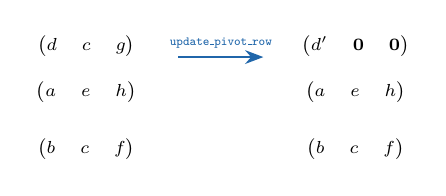
\begin{tikzpicture}[font=\scriptsize, every node/.style={transform shape}, scale=0.9]
			\node at (-1.9, 1) {$\begin{pmatrix} d & c & g \end{pmatrix}$};
			\node at (-1.9,  0.35) {$\begin{pmatrix} a & e & h \end{pmatrix}$};
			\node at (-1.9, -0.45) {$\begin{pmatrix} b & c & f \end{pmatrix}$};
			\node at ( 1.9, 1) {$\begin{pmatrix} d' & \mathbf{0} & \mathbf{0} \end{pmatrix}$};
			\node at ( 1.9,  0.35) {$\begin{pmatrix} a & e & h \end{pmatrix}$};
			\node at ( 1.9, -0.45) {$\begin{pmatrix} b & c & f \end{pmatrix}$};
			\draw[-{Stealth}, pivotblue, thick] (-0.6,0.85) -- (0.6,0.85)
		      node[midway, above] {\tiny \texttt{update\_pivot\_row}};
		\end{tikzpicture}
		
		\pause
		% -------- Update Kernel (RIGHT) ---------------------------------
		\column{0.48\textwidth}
		\begin{block}{2. Update Kernel – Apply the Transformation}
			\begin{itemize}\setlength{\itemsep}{3pt}
			  \item Receives parameters from the pivot kernel.
			  \item Applies the transformation to each trailing row.
			  \item Enables parallel execution across multiple rows.
			\end{itemize}
		\end{block}
		
		% mini-figure (two rows BEFORE → AFTER)
		\centering
		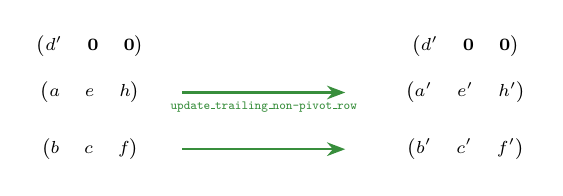
\begin{tikzpicture}[font=\scriptsize, every node/.style={transform shape}, scale=0.9]
			% before rows
			\node at (-2.1, 1) {$\begin{pmatrix} d' & \mathbf{0} & \mathbf{0} \end{pmatrix}$};
			\node at (-2.1,  0.35) {$\begin{pmatrix} a & e & h \end{pmatrix}$};
			\node at (-2.1, -0.45) {$\begin{pmatrix} b & c & f \end{pmatrix}$};
			% after rows
			\node at (3.2, 1) {$\begin{pmatrix} d' & \mathbf{0} & \mathbf{0} \end{pmatrix}$};
			\node at ( 3.2,  0.35) {$\begin{pmatrix} a' & e' & h' \end{pmatrix}$};
			\node at ( 3.2, -0.45) {$\begin{pmatrix} b' & c' & f' \end{pmatrix}$};
			% arrows
			\draw[-{Stealth}, updategreen, thick] (-0.8,  0.35) -- (1.5,  0.35)
			node[midway, below] {\tiny \texttt{update\_trailing\_non-pivot\_row}};
			\draw[-{Stealth}, updategreen, thick] (-0.8, -0.45) -- (1.5, -0.45);
		\end{tikzpicture}
	\end{columns}

	\pause
	\vspace{2mm}
	{\scriptsize \emph{The pivot kernel computes transformation parameters, which the update kernel applies to construct the upper-triangular matrix required by SLSQP.}}

\end{frame}        % The slide visualizing the kernels
	
	% --- Placeholders for the rest of the presentation ---
	% % Slide: Naive Barrier-Based Parallelism
% \begin{frame}{A Naive Approach: Parallelism with Barriers}
%   \begin{columns}[c,onlytextwidth] % Vertically center the columns

%     % ----- LEFT: The algorithm modified with a parallel loop and barriers -----
%     \column{0.55\textwidth}
%     \begin{block}{Barrier-Based Parallel Algorithm}
%       \footnotesize
%       \begin{algorithmic}[1]
%         \State \textbf{Input:} $A$, a $m \times n$ non-singular real matrix.
%         \For{$i = 1$ \textbf{to} $m$} \Comment{Outer loop remains sequential}
%           \State $(up, b) \gets \textcolor{pivotblue}{\Call{\texttt{update\_pivot\_row}}{A, i}}$
%           \State \textcolor{depred}{\textbf{--- BARRIER 1 ---}} \Comment{Wait for pivot to complete}
          
%           \ParallelFor{$j = i+1$ to $n$} \Comment{Parallelize row updates}
%             \State \textcolor{updategreen}{\Call{\texttt{update\_trailing\_non\_pivot\_row}}{A, i, j, up}}
%           \EndParallelFor
          
%           \State \textcolor{depred}{\textbf{--- BARRIER 2 ---}} \Comment{Wait for all updates to finish}
%         \EndFor
%         \State \textbf{Output:} Matrix $A$ in upper-triangular form.
%       \end{algorithmic}
%     \end{block}
% \end{columns}
%     % % ----- RIGHT: Explanation of the logic and its critical flaw -----
%     % \column{0.45\textwidth}
%     % \begin{block}{The Logic}
%     %   The most obvious way to parallelize the algorithm is to execute the inner loop across multiple threads. To maintain correctness:
%     %   \begin{itemize}
%     %     \item \textbf{Barrier 1} is needed to ensure the pivot data is ready before any thread can start an update.
%     %     \item \textbf{Barrier 2} is needed to ensure all row updates for iteration `i` are complete before we begin iteration `i+1`.
%     %   \end{itemize}
%     % \end{block}
    
%     % \begin{alertblock}{The Critical Flaw: Lost Performance}
%     %   This approach is inefficient. Threads that finish their work quickly are forced to \textbf{idle} at the barrier, waiting for the single \textbf{slowest thread} to catch up. This "tail waiting" is pure wasted time.
%     % \end{alertblock}
% \end{frame}


\begin{frame}{A Naive Approach: Parallelism with Barriers}
	
	\pause 
	\begin{columns}[c] % Vertically center the columns' content
	
	 % ----- LEFT: The algorithm -----
	 \begin{column}{0.55\textwidth}
	   \begin{block}{Barrier-Based Parallel Algorithm}
	     \footnotesize
	     \begin{algorithmic}[1]
	       \State \textbf{Input:} $A$, a $m \times n$ non-singular real matrix.
	       \For{$i = 1$ \textbf{to} $m$}
	         \State $(up, b) \gets \textcolor{pivotblue}{\Call{\texttt{update\_pivot\_row}}{A, i}}$
	         \State \textcolor{depred}{\textbf{--- BARRIER 1 ---}}
	         
	         \For{$j = i+1$ to $n$} \Comment{Parallel execution}
	           \State \textcolor{updategreen}{\Call{\texttt{update\_trailing\_non\_pivot\_row}}{A, i, j, up}}
	         \EndFor
	         
	         \State \textcolor{depred}{\textbf{--- BARRIER 2 ---}}
	       \EndFor
	       \State \textbf{Output:} Matrix $A$ in upper-triangular form.
	     \end{algorithmic}
	   \end{block}
	 \end{column}
	\end{columns}
\end{frame}
	% Slide 4 — QR as a Task DAG (Updated with simplified alertblock bullets)
\begin{frame}{Problem Formulation: QR as a Task DAG}
	
	\pause 
	
	% Use [T] to top-align the columns for better control over vertical space
	\begin{columns}[c,onlytextwidth] 
		% ---------- LEFT: Content drastically condensed into a single block ----------
		\column{0.60\textwidth}
		\begin{block}{Task \& Dependency Model}
		  The QR algorithm is modeled as a DAG of tasks, $T_{i,j}$:
		  \begin{itemize}\setlength{\itemsep}{3pt} % Tighter item spacing
		    \item \textbf{Pivot Task ($T_{i,i}$):} Runs \texttt{update\_pivot\_row}.
		    \item \textbf{Update Task ($T_{i,j}, j>i$):} Runs \texttt{update\_trailing\_non\_pivot\_row}. % FIXED: Changed &gt; to > for LaTeX compatibility
		    \item \textbf{Dependencies:} A task $T_{i,j}$ can only run after its parents, \textbf{$T_{i,i}$} (pivot) and \textbf{$T_{i-1,j}$} (previous row), are complete.
		  \end{itemize}
		\end{block}
	
		\pause 
		\begin{alertblock}{Scheduling Goal}
		  \begin{itemize}\setlength{\itemsep}{3pt} % Keep bullets tight to fit page
		    \item Execute the task DAG in parallel.
		    \item Respect all task dependencies.
		    %\item Avoid the overhead caused by global synchronization barriers.
		  \end{itemize}
		\end{alertblock}
	
		% ---- Right: TaskGraph figure with adjusted scale and caption ----		
		\column{0.40\textwidth}
		\centering
		\definecolor{lightblue}{RGB}{173, 216, 230}
		
		% --- Further reduced scale to guarantee fit ---
		\pause 
		\begin{tikzpicture}[node distance=1cm and 0.5cm, scale=0.5, transform shape]
			% Nodes - Row 1
			\node[draw, circle, fill=lightblue] (T11) at (0,0) {$T_{1,1}$};
			\node[draw, circle, fill=lightblue] (T12) at (1.4,-1.2) {$T_{1,2}$};
			\node[draw, circle] (T13) at (2.6,-1.2) {$T_{1,3}$};
			\node[draw, circle] (T14) at (3.8,-1.2) {$T_{1,4}$};
			\node[draw, circle] (T15) at (4.9,-1.2) {$T_{1,5}$};
			
			% Nodes - Row 2
			\node[draw, circle, fill=lightblue] (T22) at (1.4,-2.5) {$T_{2,2}$};
			\node[draw, circle, fill=lightblue] (T23) at (2.6,-3.5) {$T_{2,3}$};
			\node[draw, circle] (T24) at (3.8,-3.5) {$T_{2,4}$};
			\node[draw, circle] (T25) at (4.9,-3.5) {$T_{2,5}$};
			
			% Nodes - Row 3
			\node[draw, circle, fill=lightblue] (T33) at (2.6,-4.8) {$T_{3,3}$};
			\node[draw, circle, fill=lightblue] (T34) at (3.8,-5.8) {$T_{3,4}$};
			\node[draw, circle] (T35) at (4.9,-5.8) {$T_{3,5}$};
			
			% Nodes - Row 4
			\node[draw, circle, fill=lightblue] (T44) at (3.8,-7.1) {$T_{4,4}$};
			\node[draw, circle, fill=lightblue] (T45) at (4.9,-8.1) {$T_{4,5}$};
			
			% Nodes - Row 5
			\node[draw, circle, fill=lightblue] (T55) at (4.9,-9.7) {$T_{5,5}$};
			
			% Edges (condensed to save space in the .tex file)
			\draw[->] (T11) -- (T12); \draw[->] (T12) -- (T22); \draw[->] (T13) -- (T23);
			\draw[->] (T14) -- (T24); \draw[->] (T15) -- (T25); \draw[->, bend left] (T11) to (T13);
			\draw[->, bend left] (T11) to (T14); \draw[->, bend left] (T11) to (T15);
			\draw[->] (T22) -- (T23); \draw[->] (T24) -- (T34); \draw[->] (T25) -- (T35);
			\draw[->, bend left] (T22) to (T24); \draw[->, bend left] (T22) to (T25);
			\draw[->] (T23) -- (T33); \draw[->, bend left] (T33) to (T34); \draw[->, bend left] (T33) to (T35);
			\draw[->] (T34) -- (T44); \draw[->] (T35) -- (T45); \draw[->, bend left] (T44) to (T45);
			\draw[->] (T45) -- (T55);
		\end{tikzpicture}
		
		% --- Added the requested figure caption ---
		\vspace{1mm}
		{\scriptsize \emph{TaskGraph for Triangular System}}
	
	\end{columns}
\end{frame}
 % FIXED: Added missing .tex extension (was QrAsDag in original)
	% Slide: Barrier-Based Task Scheduling
\begin{frame}{A Simple Approach: Barriers on a Task Graph}
  \begin{columns}[c,onlytextwidth] % Vertically center the columns

    % ----- LEFT: Explanation of the barrier logic for tasks -----
    \column{0.50\textwidth}
    \begin{block}{The Barrier-Based Approach}
      A straightforward way to parallelize the QR algorithm is to first model it as a graph of tasks ($T_{i,j}$) and then use barriers to enforce dependencies:
      \begin{itemize}
        \item \textbf{Barrier 1:} After the pivot task \textcolor{pivotblue}{$T_{i,i}$} completes, all threads must wait. This ensures the transformation info is available.
        \item \textbf{Barrier 2:} After all parallel update tasks \textcolor{updategreen}{$T_{i,j}$} are done, all threads must wait again before starting the next iteration ($i+1$).
      \end{itemize}
    \end{block}
    


    % ----- RIGHT: The TikZ figure illustrating the problem -----
    \column{0.45\textwidth}
          \begin{alertblock}{The Critical Flaw: Wasted Time}
      Barriers impose a rigid, synchronous execution. Threads that finish their tasks early are forced to \textbf{idle}, waiting for the single \textbf{slowest thread} to catch up. This "tail waiting" is pure computational waste.
    \end{alertblock}
    % --- Rescaled and re-dimensioned the TikZ figure to prevent overflow ---
    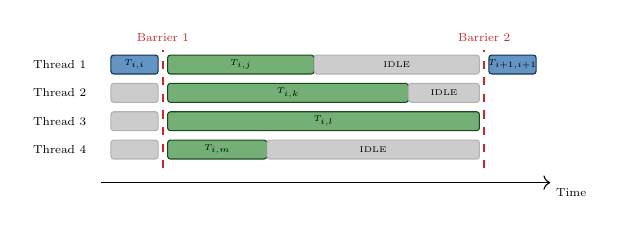
\begin{tikzpicture}[font=\tiny, every node/.style={transform shape}, scale=0.60]
      % Styles for different states
      \tikzset{pivot/.style={fill=pivotblue!70, draw=pivotblue!50!black, rounded corners=1pt}}
      \tikzset{work/.style={fill=updategreen!70, draw=updategreen!50!black, rounded corners=1pt}}
      \tikzset{wait/.style={fill=gray!40, draw=gray!60, rounded corners=1pt}}
      \tikzset{bar/.style={draw=depred, thick, dashed}}

      % Time Axis
      \draw[->] (0,0) -- (9.5,0) node[anchor=north west, font=\scriptsize] {Time};
      
      % Thread Labels
      \node[anchor=east, font=\scriptsize] at (-0.2, 2.5) {Thread 1};
      \node[anchor=east, font=\scriptsize] at (-0.2, 1.9) {Thread 2};
      \node[anchor=east, font=\scriptsize] at (-0.2, 1.3) {Thread 3};
      \node[anchor=east, font=\scriptsize] at (-0.2, 0.7) {Thread 4};

      % --- Iteration i with new, narrower coordinates ---
      \draw[pivot] (0.2, 2.3) rectangle node{$T_{i,i}$} (1.2, 2.7);
      \draw[wait]  (0.2, 1.7) rectangle (1.2, 2.1);
      \draw[wait]  (0.2, 1.1) rectangle (1.2, 1.5);
      \draw[wait]  (0.2, 0.5) rectangle (1.2, 0.9);
      \node[above=2pt, depred, font=\scriptsize] at (1.3, 2.8) {Barrier 1};
      \draw[bar] (1.3, 0.3) -- (1.3, 2.8);

      \draw[work] (1.4, 2.3) rectangle node{$T_{i,j}$} (4.5, 2.7);
      \draw[work] (1.4, 1.7) rectangle node{$T_{i,k}$} (6.5, 2.1);
      \draw[work] (1.4, 1.1) rectangle node{$T_{i,l}$} (8.0, 1.5); % SLOWEST
      \draw[work] (1.4, 0.5) rectangle node{$T_{i,m}$} (3.5, 0.9);

      \draw[wait] (4.5, 2.3) rectangle node{\textcolor{black}{IDLE}} (8.0, 2.7);
      \draw[wait] (6.5, 1.7) rectangle node{\textcolor{black}{IDLE}} (8.0, 2.1);
      \draw[wait] (3.5, 0.5) rectangle node{\textcolor{black}{IDLE}} (8.0, 0.9);
      
      \node[above=2pt, depred, font=\scriptsize] at (8.1, 2.8) {Barrier 2};
      \draw[bar] (8.1, 0.3) -- (8.1, 2.8);

      \draw[pivot] (8.2, 2.3) rectangle node{$T_{i+1,i+1}$} (9.2, 2.7);
    \end{tikzpicture}
    
    % --- Added the requested figure caption ---
    \vspace{2mm}
    {\scriptsize \emph{Barrier scheduling forces fast threads to wait, causing idle time.}}
  \end{columns}
\end{frame} % FIXED: Capitalization to match file name
	% Slide: Two-Queue Approach (Introduction - Flow Logic, Final Corrected Layout)
\begin{frame}{Our Solution: Asynchronous Two-Queue Scheduling}
  \vspace{-3mm}
  \begin{minipage}[c][\textheight][c]{0.45\textwidth}
    \vspace*{\fill}
    \begin{block}{The Problem with Barriers}
      Barriers are inefficient because they force fast threads to idle. The key to better performance is to eliminate this synchronous waiting.
    \end{block}

    \begin{alertblock}{The Two-Queue Solution}
      Our approach replaces global barriers with two shared, lock-free queues that manage the flow of tasks based on their readiness:
      \begin{itemize}
        \item \textbf{\alert{Main Queue}:} Holds tasks that are ready for execution.
        \item \textbf{\alert{Wait Queue}:} A holding area for tasks with unmet dependencies.
      \end{itemize}
    \end{alertblock}
    \vspace*{\fill}
  \end{minipage}
  \hfill
  \begin{minipage}[c][\textheight][c]{0.5\textwidth}
    \vspace*{\fill}
    \centering
    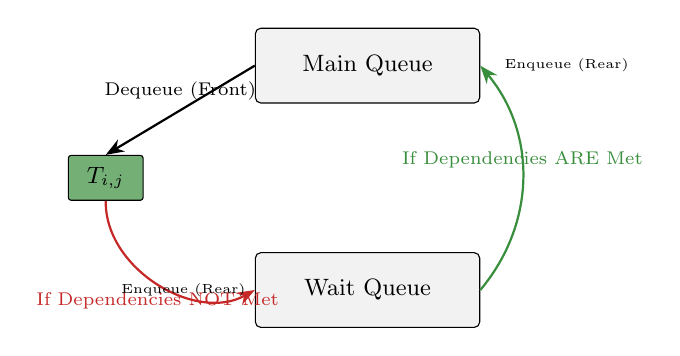
\begin{tikzpicture}[font=\small, every node/.style={transform shape}, scale=0.95]
      % Styles
      \tikzset{queue/.style={draw, rectangle, minimum width=3cm, minimum height=1cm, rounded corners=2pt, fill=gray!10, align=center}}
      \tikzset{task/.style={draw, rectangle, rounded corners=1pt, fill=updategreen!70, minimum width=1cm, minimum height=0.6cm}}
      \tikzset{arrow_label/.style={align=center, font=\scriptsize}}
      
      % --- The Queues, positioned vertically on the right ---
      \node[queue] (main) at (0, 1.5) {Main Queue};
      \node[queue] (wait) at (0, -1.5) {Wait Queue};
      
      % --- The Dequeued Task, on the left ---
      \node[task] (task_out) at (-3.5, 0) {$T_{i,j}$};
      
      % --- The Arrows with Corrected Paths and Labels ---
      % 1. Dequeue from Main Queue
      \draw[-{Stealth}, thick] (main.west) -- node[above, arrow_label] {Dequeue (Front)} (task_out.north);
      
      % 2. Move to Wait Queue if not ready
      \draw[-{Stealth}, thick, depred] (task_out.south) to[bend right=60] 
        node[below, arrow_label] {If Dependencies NOT Met} (wait.west);
      \node[anchor=east, font=\tiny] at (wait.west) {\hspace{10mm}Enqueue (Rear)};

      % 3. Promote from Wait Queue if ready
      \draw[-{Stealth}, thick, updategreen] (wait.east) to[bend right=40] 
        node[above, arrow_label] {If Dependencies ARE Met} (main.east);
      \node[anchor=west, font=\tiny] at (main.east) {\hspace{2mm}Enqueue (Rear)};

    \end{tikzpicture}
    \vspace*{\fill}
  \end{minipage}

\end{frame}
	\begin{frame}{Simulation: Execution \& Spawning}
  \begin{columns}[c,onlytextwidth]

    % ----- LEFT: Text that updates with each click -----
    \column{0.4\textwidth}
    \only<1>{
      \begin{alertblock}{Step 1: Initial Task}
        The system starts with \textbf{$T_{1,1}$} ready at the front of the Main Queue.
      \end{alertblock}
    }
    \only<2-3>{
      \begin{alertblock}{Step 2: Dequeue \& Execute}
        An available thread, \textbf{T1}, from the pool dequeues the task from the Main Queue.
      \end{alertblock}
    }
    \only<4->{
      \begin{alertblock}{Step 3: Enqueue Children}
        After executing the task, T1 enqueues the ready child tasks (with dependencies satisfied) $T_{1,2}, \dots$ to the Main Queue.
      \end{alertblock}
    }

    % ----- RIGHT: The diagram with polished, non-overlapping arrows -----
    \column{0.6\textwidth}
    \centering
    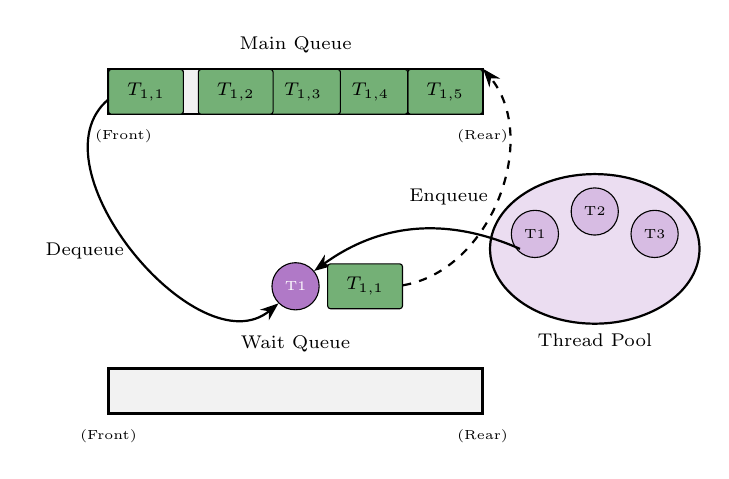
\begin{tikzpicture}[font=\scriptsize, every node/.style={transform shape}, scale=0.95]
      % Styles
      \tikzset{pool/.style={draw, thick, ellipse, fill=accent!15, minimum width=2.8cm, minimum height=2cm}}
      \tikzset{thread_icon/.style={draw, circle, fill=accent!30, minimum size=0.5cm}}
      \tikzset{active_thread/.style={thread_icon, fill=accent!60, text=white, minimum size=0.6cm}}
      \tikzset{task_ready/.style={draw, rectangle, rounded corners=1pt, fill=updategreen!70, minimum width=1cm, minimum height=0.6cm}}
      \tikzset{queue_box/.style={draw, thick, fill=gray!10}}
      
      % --- Layout Elements ---
      \node[pool] (pool) at (3.5, 0) {};
      \node[anchor=north] at (pool.south) {Thread Pool};
      \node[anchor=south] at (-0.5, 2.5) {Main Queue};
      \draw[queue_box] (-3, 1.8) rectangle (2, 2.4);
      \node[font=\tiny] at (-2.8, 1.5) {(Front)};
      \node[font=\tiny] at (2, 1.5) {(Rear)};
      \node[anchor=south] at (-0.5, -1.5) {Wait Queue};
      \draw[queue_box] (-3, -2.2) rectangle (2, -1.6);
      \node[font=\tiny] at (-3, -2.5) {(Front)};
      \node[font=\tiny] at (2, -2.5) {(Rear)};
      
      % --- Idle Threads in the Pool ---
      \node<1,4->[thread_icon] at ($(pool.center)+(-0.8,0.2)$) {\tiny T1}; 
      \node[thread_icon] at ($(pool.center)+(0,0.5)$) {\tiny T2};
      \node[thread_icon] at ($(pool.center)+(0.8,0.2)$) {\tiny T3};
      
      % --- ANIMATION SEQUENCE ---
      
      % 1. Initial State
      \node<1>[task_ready] at (-2.5, 2.1) {$T_{1,1}$};
      
      % 2. T1 moves out of the pool
      \node<2-3>[active_thread] (active_t1) at (-0.5, -0.5) {\tiny T1};
      \draw<2>[-{Stealth}, thick] ($(pool.center)+(-1,0)$) to[bend right] (active_t1);
      
      % 3. T1 dequeues the task
      \node<2>[task_ready] at (-2.5, 2.1) {$T_{1,1}$};
      \node<3->[task_ready, right=1mm of active_t1] (task_t11) {$T_{1,1}$};
      % --- FIX 1: Increased bend to arc over the "(Front)" text ---
      \draw<3>[-{Stealth}, thick] (-3, 2.0) to[bend right=90] node[midway, left] {Dequeue} (active_t1);
      
      % 4. T1 enqueues the children
      % The new tasks appear at the Rear
      \node<4->[task_ready] at (1.5, 2.1) (t15) {$T_{1,5}$};
      \node<4->[task_ready] at (0.5, 2.1)  {$T_{1,4}$};
      \node<4->[task_ready] at (-0.4, 2.1) {$T_{1,3}$};
      \node<4->[task_ready] at (-1.3, 2.1) {$T_{1,2}$};
      % --- FIX 2: Draw the arrow AFTER the tasks so it appears on top ---
      \draw<4>[dashed, -{Stealth}, thick] (task_t11) to[bend right=60] node[midway, left] {Enqueue} (t15.north east);

    \end{tikzpicture}
  \end{columns}
\end{frame}
	\begin{frame}{Simulation: The Two-Queue Scheduler in Action}
  \begin{columns}[c,onlytextwidth] % Vertically centered

    % ----- LEFT: The text explaining State B -----
    \column{0.4\textwidth}
    \begin{alertblock}{State B: Execution \& Spawning}
      An idle thread, \textbf{T1}, dequeues the pivot task \textbf{$T_{1,1}$} from the \textbf{front} of the Main Queue.
      \vspace{2mm}
      
      After executing it, T1 enqueues the newly spawned, ready-to-run child tasks (\textbf{$T_{1,2}, T_{1,3}, \dots$}) to the \textbf{rear} of the Main Queue.
    \end{alertblock}

    % ----- RIGHT: The diagram showing the action of State B -----
    \column{0.6\textwidth}
    \centering
    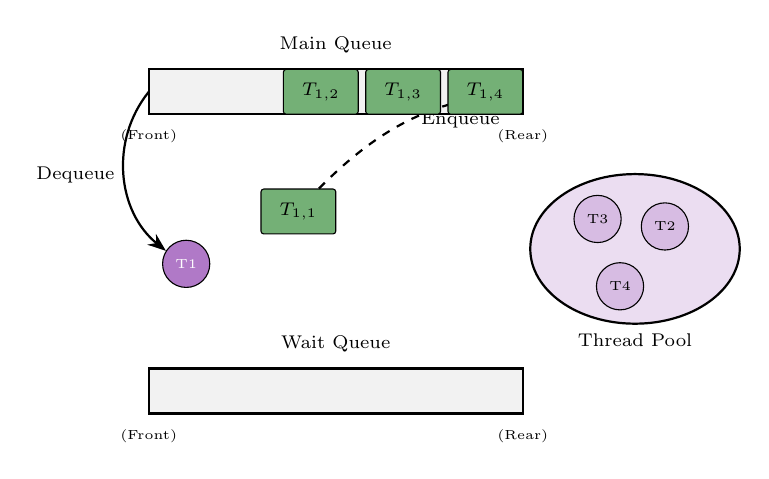
\begin{tikzpicture}[font=\scriptsize, every node/.style={transform shape}, scale=0.95]
      % Styles
      \tikzset{pool/.style={draw, thick, ellipse, fill=accent!15, minimum width=2.8cm, minimum height=2cm, align=center}}
      \tikzset{thread_icon/.style={draw, circle, fill=accent!30, minimum size=0.5cm}}
      \tikzset{active_thread/.style={thread_icon, fill=accent!60, text=white, minimum size=0.6cm}}
      \tikzset{task_ready/.style={draw, rectangle, rounded corners=1pt, fill=updategreen!70, minimum width=1cm, minimum height=0.6cm}}
      \tikzset{queue_box/.style={draw, thick, fill=gray!10}}
      
      % --- Repositioned Elements for Clarity ---
      % Main Queue at the top
      \node[anchor=south] at (-0.5, 2.5) {Main Queue};
      \draw[queue_box] (-3, 1.8) rectangle (2, 2.4);
      \node[font=\tiny] at (-3, 1.5) {(Front)};
      \node[font=\tiny] at (2, 1.5) {(Rear)};

      % Wait Queue at the bottom
      \node[anchor=south] at (-0.5, -1.5) {Wait Queue};
      \draw[queue_box] (-3, -2.2) rectangle (2, -1.6);
      \node[font=\tiny] at (-3, -2.5) {(Front)};
      \node[font=\tiny] at (2, -2.5) {(Rear)};

      % Thread Pool on the right (T1 is missing)
      \node[pool] (pool) at (3.5, 0) {};
      \node[thread_icon] at ($(pool.center)+(0.4,0.3)$) {\tiny T2};
      \node[thread_icon] at ($(pool.center)+(-0.5, 0.4)$) {\tiny T3};
      \node[thread_icon] at ($(pool.center)+(-0.2, -0.5)$) {\tiny T4};
      \node[anchor=north] at (pool.south) {Thread Pool};

      % --- Active T1 and its task are in the center-left "workspace" ---
      \node[active_thread] (active_t1) at (-2.5, -0.2) {\tiny T1};
      \node[task_ready] (task_t11) at (-1, 0.5) {$T_{1,1}$};

      % --- The Actions (Clear, Curved Arrows) ---
      % Dequeue Arrow: from Front of Queue to the active T1
      \draw[-{Stealth}, thick] (-3, 2.1) to[bend right=45] node[midway, left] {Dequeue} (active_t1);
      
      % Enqueue Arrow: from the processed task to the Rear of Queue
      \draw[-{Stealth}, thick, dashed] (task_t11) to[bend left=20] node[midway, right] {Enqueue} (2, 2.1);
      
      % --- The Result: New tasks are now in the Main Queue ---
      \node[task_ready] at (1.5, 2.1) {$T_{1,4}$};
      \node[task_ready] at (0.4, 2.1) {$T_{1,3}$};
      \node[task_ready] at (-0.7, 2.1) {$T_{1,2}$};
      
    \end{tikzpicture}
  \end{columns}
\end{frame}
	% Simulation Slide 3, Step 1: The Initial State (Final Revised Version)
\begin{frame}{Simulation: Navigating the Dependency Graph}
  \begin{columns}[c,onlytextwidth]

    % ----- LEFT: Text for the initial state -----
    \column{0.38\textwidth}
    \only<1>{
      \begin{alertblock}{Mid-Execution Step}
      After executing $T_{2, 2}$ its children's dependencies are checked and enqueued to the main queue if its dependency is satisfied or else its enqueued into the wait queue.
        
      \end{alertblock}
    }
    \only<2>{
      \begin{alertblock}{Step 5: Dependency Aware Enqueue Process}
        Thread \textbf{T3} is processing its task from the previous level.
        So the children task $T_{2, 4}$ gets pushed to the wait queue as its parent task is incomplete.
      \end{alertblock}
    }
    \only<3>{
      \begin{alertblock}{Step 6: Continued Execution with Readily Available Tasks}
        The remaining threads can pick up other immediately executable tasks from the main queue.
      \end{alertblock}
    }
        \only<4>{
      \begin{alertblock}{Step 7: Next Pivot Push}
        \textbf{T1} finishes $T_{2, 3}$ and enqueues its child, the new pivot \textbf{$T_{3,3}$}. Also, $T_{1, 4}$ is complete in the mean time so its child $T_{2, 4}$ can be safely pushed to the main queue.
    \end{alertblock}
    }
        \only<5>{
      \begin{alertblock}{Step 8: Promotion Admist Work}
        Since, the parent of $T_{2, 4}$ was complete, $T_{2, 4}$ got promoted from the wait queue to the main queue as an immediately executable task.
      \end{alertblock}
    }

        \only<6>{
      \begin{alertblock}{Step 9: Further Execution with Immediately Executable Tasks}
        The threads can pick up more executable tasks from the main queue and continue executing the nodes of the DAG in a non-blocking manner.
      \end{alertblock}
    }


    % ----- RIGHT: The static diagram with your new layout and dashed arrows -----
    \column{0.61\textwidth}
    \centering
    \begin{tikzpicture}[font=\scriptsize, every node/.style={transform shape}, scale=0.95]
      % Styles
      \tikzset{pool/.style={draw, thick, ellipse, fill=accent!15, minimum width=2.8cm, minimum height=2cm}}
      \tikzset{thread_icon/.style={draw, circle, fill=accent!30, minimum size=0.5cm}}
      \tikzset{active_thread/.style={thread_icon, fill=accent!60, text=white, minimum size=0.6cm}}
      \tikzset{task_ready/.style={draw, rectangle, rounded corners=1pt, fill=updategreen!70, minimum width=1cm, minimum height=0.6cm}}
      \tikzset{task_wait/.style={draw, rectangle, rounded corners=1pt, fill=gray!50, minimum width=1cm, minimum height=0.6cm}}
      \tikzset{queue_box/.style={draw, thick, fill=gray!10, minimum width=5cm, minimum height=0.8cm}}
      
      % --- Layout Elements ---
      \node[pool] (pool) at (3.5, 0) {}; \node[anchor=north] at (pool.south) {Thread Pool};
      \node[queue_box] (mainq) at (-0.5, 2.1) {}; \node[anchor=south] at (mainq.north) {Main Queue};
      \node[font=\tiny] at ([yshift=-0.3cm]mainq.south west) {(Front)}; \node[font=\tiny] at ([yshift=-0.3cm]mainq.south east) {(Rear)};
      \node[queue_box] (waitq) at (-0.5, -2.1) {}; \node[anchor=north] at ([yshift=0.4cm]waitq.north) {Wait Queue};
      \node[font=\tiny] at ([yshift=-0.3cm]waitq.south west) {Front)}; \node[font=\tiny] at ([yshift=-0.3cm]waitq.south east) {(Rear)};
      
      % --- Initial State Elements ---
       \only<1>{
      % Active Threads (T3 and T4)
      \node[active_thread] (t3) at (0, 0.7) {\tiny T3}; \node[task_ready, right=1mm of t3] {$T_{1,4}$};
      \node[active_thread] (t4) at (0, -0.7) {\tiny T4}; \node[task_ready, right=1mm of t4] {$T_{1,5}$};
      
      \node[thread_icon] (t2_idle) at ($(pool.center)+(0,0.5)$) {\tiny T2};
      
      % Tasks in Main Queue
      \node[task_ready] (t22_q) at ([xshift=-1.8cm]mainq.center) {$T_{2,2}$};
          \node[active_thread] (active_t1) at (-2.5, -0.7) {\tiny T1};
        \draw[-{Stealth}, thick] (mainq.west) to[bend right=60] node[midway, left] {Dequeue} (active_t1);

      }


 % --- STATE 2 (After First Click - Corrected) ---


      % --- STATE 3 (After Second Click - Corrected) ---
      \only<2>{
        % T3 is still active, executing the parent task
        \node[active_thread] (t3) at (0, 0.7) {\tiny T3}; \node[task_ready, right=1mm of t3] {$T_{1,4}$};
        \node[active_thread] (active_t2) at (-2.5, -0.7) {\tiny T1};
        % The fail arrow appears, and T2,4 moves to the Wait Queue
    
        \node[task_wait] (t24_q)at ([xshift=1.8cm]waitq.center) {$T_{2,4}$};
        \draw[-{Stealth}, thick, depred, dashed] (active_t2) to[out=180, in=220] 
        node[midway, below left] {Fail} (t24_q.south);
        \node[task_ready] (t23_q) at ([xshift=0.6cm]mainq.west) {$T_{2,3}$};
        \node[task_ready] (t25_q) at ([xshift=1.6cm]mainq.west) {$T_{2,5}$};
          \node[thread_icon] (t4_idle) at ($(pool.center)+(0,-0.5)$) {\tiny T4};
        \node[thread_icon] (t2_idle) at ($(pool.center)+(0,0.5)$) {\tiny T2};   
         \draw[-{Stealth}, thick, dashed] (active_t1) to[bend right=60] 
        node[midway, below right] {Pass} (t25_q.east);

      }
      % --- STATE 4 (After Third Click) ---
      \only<3>{
        \node[active_thread] (t3) at (0, 0.7) {\tiny T3}; \node[task_ready, right=1mm of t3] {$T_{1,4}$};
        \node[thread_icon] at ($(pool.center)+(0.8,0.2)$) {\tiny T4};
       
        \node[active_thread] (active_t1) at (-2.5, -0.7) {\tiny T1};
        \draw[-{Stealth}, thick] (mainq.west) to[bend right=60] node[midway, left] {Dequeue} (active_t1);

        \node[active_thread] (active_t2) at (-1.5, -0.7) {\tiny T2};
        
        \node[task_ready] (t23_q) at ([xshift=0.6cm]mainq.west) {$T_{2,3}$};

        \node[task_ready] (t25_q) at ([xshift=1.6cm]mainq.west) {$T_{2,5}$};
    
        % T2,4 is still in the Wait Queue
        \node[task_wait] at ([xshift=1.8cm]waitq.center) {$T_{2,4}$};
        
      \draw[-{Stealth}, thick] (t25_q.east) to[bend left=60]  (active_t2);
      }
      % --- STATE 5 (After Fourth Click) ---
      \only<4>{
       

        \node[thread_icon] at ($(pool.center)+(0.8,0.2)$) {\tiny T3};
        \node[thread_icon] at ($(pool.center)+(-0.5,-0.5)$) {\tiny T4};
        \node[active_thread] (active_t2) at (-2.5, -0.7) {\tiny T2};
        \node[task_ready, right=1mm of active_t2] {$T_{2,5}$};

        \node[task_ready] at ([xshift=-0.8cm]mainq.east) {$T_{3,3}$};

        \node[active_thread] (t3) at (0, 0.7) {\tiny T1}; 
        \draw[-{Stealth}, thick] (0.3, 0.7) to[bend right=30] node[midway, right] {enqueue}([xshift=1.4cm]mainq.south);
        
        \node[task_ready] at ([xshift=0.8cm]waitq.west) {$T_{2,4}$};
      }

      \only<5>{
        % T1 and T3 are idle

        \node[thread_icon] at ($(pool.center)+(0.8,0.2)$) {\tiny T4};
        \node[thread_icon] at ($(pool.center)+(0.1,0.2)$) {\tiny T2};

        \node[active_thread] (active_t2) at (-2.5, -0.7) {\tiny T1};

        \draw[-{Stealth}, thick, updategreen, dashed] (waitq.west) to[bend left =45] (active_t2);
        \draw[-{Stealth}, thick, updategreen, dashed] (active_t2) to[bend right=30] node[midway, left] {Promote} ([xshift = 1.6cm]mainq.south);
        \node[task_ready] at ([xshift=1.8cm]mainq.center) {$T_{2,4}$};

      \node[active_thread] (t4) at (0, -0.7) {\tiny T3}; \node[task_ready, right=1mm of t4] {$T_{3,3}$};
      }

      % --- STATE 7 (After Sixth Click) ---
    \only<6->{
        % Idle threads remaining in the pool
        \node[thread_icon] at ($(pool.center)+(-0.8,0.2)$) {\tiny T3};
        
        % T2 and T4 are now active, taking the NEW work
        \node[active_thread] (active_t2) at (-2.5, -0.7) {\tiny T1};
        \node[active_thread] (active_t1) at (0, -0.7) {\tiny T4};
        \node[active_thread] (active_t3) at (-3.5, 0.7) {\tiny T2};
        
        % Arrows showing T2 and T4 dequeuing the new tasks
        \draw[-{Stealth}, thick] ([xshift=0.4cm]mainq.center) to[bend right = 15] (active_t2);
        \draw[-{Stealth}, thick] ([xshift=1.8cm]mainq.center) to[bend right] (active_t1);
        \draw[-{Stealth}, thick] ([xshift=0.4cm]mainq.west) to[bend right = 45] (active_t3);
        % T3 has implicitly finished T3,3 and enqueued its children
        % The children are now in the main queue
        \node[task_ready] at ([xshift=0.4cm]mainq.center) {$T_{3,4}$};
        \node[task_ready] at ([xshift=1.8cm]mainq.center) {$T_{3,5}$};
        
        % T2,4 is also still in the queue, ready to be picked up
        \node[task_ready] at ([xshift=-1.8cm]mainq.center) {$T_{2,4}$};
        
        }
      
\end{tikzpicture}
\end{columns}
\end{frame}
	% New Slide: Experimental Setup
\begin{frame}{Experimental Setup \& Configurations}

	\pause
	\begin{block}{The Goal of Our Experiments}
		We conducted a series of experiments to answer three key questions:
		\begin{itemize}
			\item How do we find the optimal task granularity ($\alpha, \beta$)?
			\item How does our two-queue scheduler scale compared to the barrier scheduling?
			\item What is the final, end-to-end impact on the SLSQP solver?
		\end{itemize}
	\end{block}
	
	\pause
	\begin{alertblock}{Implementation \& Configurations}
		We used Intel Threading Building Blocks (TBB) library for scheduling.
		\vspace{1mm}
		
		We evaluate two primary configurations of our scheduler:
		\begin{itemize}
			\item \textbf{Without Priority:} Uses TBB's "concurrent\_queue". Tasks are processed in a first-in, first-out (FIFO) order.
			\item \textbf{With Priority:} Uses TBB's "concurrent\_priority\_queue". Tasks on the critical path are assigned higher priority to be executed sooner.
		\end{itemize}
	\end{alertblock}

\end{frame}
	% Slide: Defining alpha, beta, and Priority (Corrected Layout)
\begin{frame}{Tuning for Performance: Granularity \& Priority}

	\begin{columns}[T,onlytextwidth]
	% ----- LEFT: Defining alpha and beta -----
	
	\pause 
	\column{0.45\textwidth}
	\begin{block}{Task Granularity}
	  We tune two parameters to control the amount of work per task:
	  \begin{itemize}
	    \item \textbf{$\alpha$}: Number of pivots per task.
	    \item \textbf{$\beta$}: Number of row updates per task.
	  \end{itemize}
	\end{block}
	
	\begin{alertblock}{The Trade-off}
	  \centering
	  \large
	  Small $(\alpha, \beta)$ \quad vs. \quad Large $(\alpha, \beta)$ \\
	  \small
	  (More Overhead) \quad (Load Imbalance)
	\end{alertblock}
	
	% ----- RIGHT: Explaining Priority Assignment -----
	\pause 
	\column{0.45\textwidth}
	\begin{block}{Priority Scheduling}
	  We prioritize tasks based on their \textbf{Bottom Level} (`bottomL`) in the DAG.
	  \begin{itemize}
	    \item Tasks on the critical path have the highest priority and are executed first.
	  \end{itemize}
	\end{block}
	
	\begin{alertblock}{The Cost of Priority}
	  Priority queues have overhead from rebalancing. This cost is:
	  \begin{itemize}
	    \item \textbf{High} for many small tasks.
	    \item \textbf{Low} for fewer large tasks.
	  \end{itemize}
	\end{alertblock}
	
	\end{columns}
\end{frame}
        % Slide: Priority Scheduling & Performance Trade-offs (Revised)
\begin{frame}{Priority Scheduling \& Performance Trade-offs}

  \begin{block}{Prioritizing the Critical Path}
    To further improve performance, we can execute more important tasks first.
    \begin{itemize}
      \item Inspired by the work of \textbf{Baskaran et al.}, we assign each task a priority.
      \item The priority is based on the task's \textbf{Bottom Level} (`bottomL`)—the longest path of work remaining from that task.
      \item This forces tasks on the \textbf{critical path} to be 
      scheduled sooner, potentially unlocking more parallelism.
    \end{itemize}
  \end{block}

  \begin{alertblock}{The Trade-off: Granularity vs. Overhead}
    The effectiveness of the priority queue depends on the task size $(\alpha, \beta)$:
    \begin{itemize}
      \item \textbf{Many small tasks:} High overhead from frequent queue rebalancing.
      \item \textbf{Fewer large tasks:} Low overhead, allowing the benefit of priority ordering to dominate.
    \end{itemize}
  \end{alertblock}

\end{frame}
	% Slide: Heatmap Results
\begin{frame}{Tuning Results: Heatmaps}

	\begin{columns}[c,onlytextwidth]
		% ----- LEFT: Without Priority -----		
		\pause 
		\column{0.40\textwidth}
		\begin{figure}
		  \centering
		  \includegraphics[width=\textwidth]{heatmap_without_priority.png}
		  \caption{\textbf{Without Priority:} Optimal performance with smaller task chunks, at $(\alpha, \beta) \approx (12, 12)$.}
		\end{figure}
		
		% ----- RIGHT: With Priority -----
		\column{0.40\textwidth}
		\pause
		\begin{figure}
		  \centering
		  \includegraphics[width=\textwidth]{heatmap_with_priority.png}
		  \caption{\textbf{With Priority:} Optimal performance with larger task chunks, at $(\alpha, \beta) \approx (30, 30)$, to reduce priority queue overhead.}
		\end{figure}
	\end{columns}
  
\end{frame}
	% Slide: Bar Chart Results
\begin{frame}{Tuning Results: Optimal Values vs. Matrix Size}
	
	\begin{figure}
		\centering
		% NOTE: This uses the PGFPlots code from your expts.tex file
		% First bar chart
		\pause 
		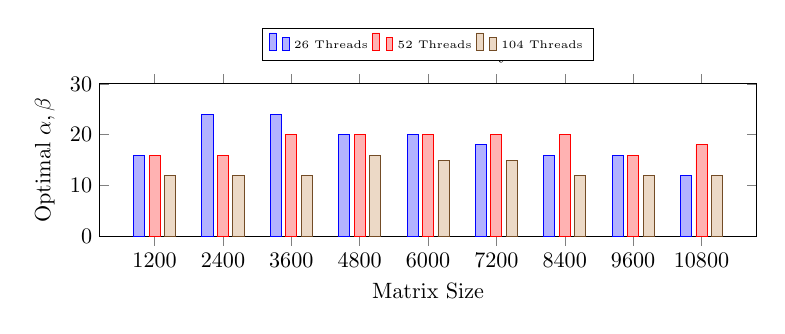
\begin{tikzpicture}[scale=0.8, transform shape]
		  \begin{axis}[
		      title={Without Priority},
		      ybar,
		      bar width=5pt,
		      symbolic x coords={1200,2400,3600,4800,6000,7200,8400,9600,10800},
		      xtick=data,
		      xlabel={Matrix Size},
		      ylabel={Optimal $\alpha, \beta$},
		      legend style={at={(0.5,1.15)}, anchor=south, legend columns=-1, font=\tiny},
		      ymin=0, ymax=30,
		      width=12cm, height=4cm
		      ]
		      \addplot coordinates {(1200,16) (2400,24) (3600,24) (4800,20) (6000,20) (7200,18) (8400,16) (9600,16) (10800,12)};
		      \addplot coordinates {(1200,16) (2400,16) (3600,20) (4800,20) (6000,20) (7200,20) (8400,20) (9600,16) (10800,18)};
		      \addplot coordinates {(1200,12) (2400,12) (3600,12) (4800,16) (6000,15) (7200,15) (8400,12) (9600,12) (10800,12)};
		      \legend{26 Threads, 52 Threads, 104 Threads}
		  \end{axis}
		\end{tikzpicture}
		
		\vspace{4mm}
		\pause 
		% Second bar chart
		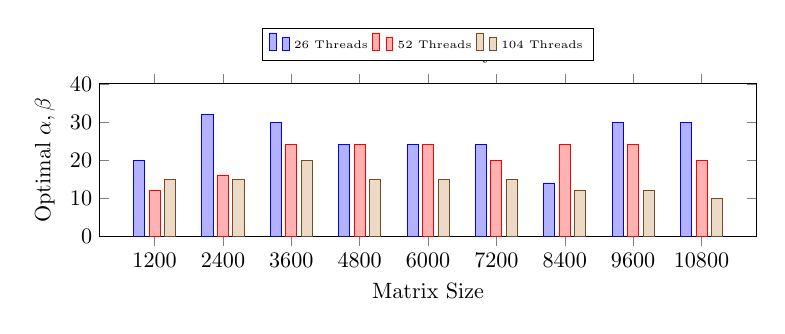
\begin{tikzpicture}[scale=0.8, transform shape]
		  \begin{axis}[
		      title={With Priority},
		      ybar,
		      bar width=5pt,
		      symbolic x coords={1200,2400,3600,4800,6000,7200,8400,9600,10800},
		      xtick=data,
		      xlabel={Matrix Size},
		      ylabel={Optimal $\alpha, \beta$},
		      legend style={at={(0.5,1.15)}, anchor=south, legend columns=-1, font=\tiny},
		      ymin=0, ymax=40,
		      width=12cm, height=4cm
		      ]
		      \addplot coordinates {(1200,20) (2400,32) (3600,30) (4800,24) (6000,24) (7200,24) (8400,14) (9600,30) (10800,30)};
		      \addplot coordinates {(1200,12) (2400,16) (3600,24) (4800,24) (6000,24) (7200,20) (8400,24) (9600,24) (10800,20)};
		      \addplot coordinates {(1200,15) (2400,15) (3600,20) (4800,15) (6000,15) (7200,15) (8400,12) (9600,12) (10800,10)};
		      \legend{26 Threads, 52 Threads, 104 Threads}
		  \end{axis}
		\end{tikzpicture}
	\end{figure}
  
\end{frame}
	% Slide: Scalability with Matrix Size (Corrected Layout)
\begin{frame}{Results: Scalability with Matrix Size}

  \begin{columns}[T] % Top-align the columns

    % ----- LEFT: 26 Threads -----
    \pause
    \column{0.5\textwidth}
    \centering    
    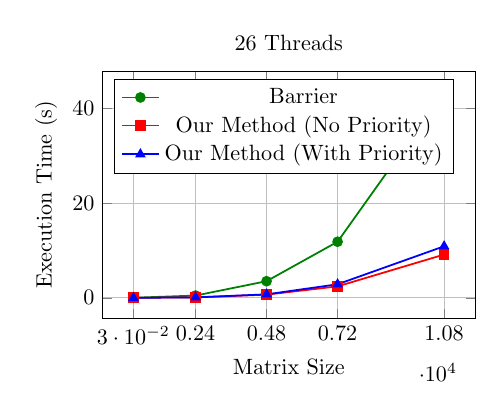
\begin{tikzpicture}[scale=0.8, transform shape]
      \begin{axis}[
          title={26 Threads},
          xlabel={Matrix Size},
          ylabel={Execution Time (s)},
          xtick={300, 2400, 4800, 7200, 10800},
          legend pos=north west,
          grid=major,
          width=7.5cm,
          height=5.5cm % Reduced height
          ]
          \addplot[darkgreen, mark=*, thick] coordinates { (300,0.009) (2400,0.472) (4800,3.507) (7200,11.838) (10800,43.428) };
          \addlegendentry{Barrier};
          \addplot[red, mark=square*, thick] coordinates { (300,0.002) (2400,0.089) (4800,0.669) (7200,2.416) (10800,9.132) };
          \addlegendentry{Our Method (No Priority)};
          \addplot[blue, mark=triangle*, thick] coordinates { (300,0.002) (2400,0.087) (4800,0.731) (7200,2.857) (10800,10.879) };
          \addlegendentry{Our Method (With Priority)};
      \end{axis}
    \end{tikzpicture}

    % ----- RIGHT: 52 Threads -----
    \pause
    \column{0.5\textwidth}
    \centering
    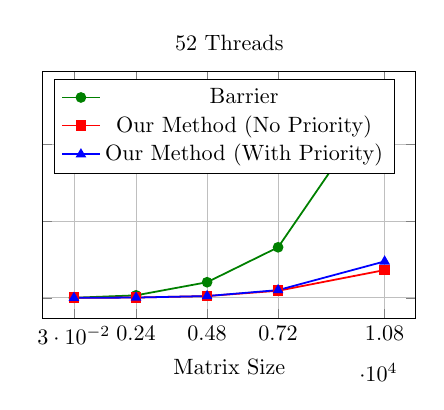
\begin{tikzpicture}[scale=0.8, transform shape]
      \begin{axis}[
          title={52 Threads},
          xlabel={Matrix Size},
          yticklabels={,,},
          xtick={300, 2400, 4800, 7200, 10800},
          legend pos=north west,
          grid=major,
          width=7.5cm,
          height=5.5cm % Reduced height
          ]
          \addplot[darkgreen, mark=*, thick] coordinates { (300,0.013) (2400,0.646) (4800,4.058) (7200,13.150) (10800,53.541) };
          \addlegendentry{Barrier};
          \addplot[red, mark=square*, thick] coordinates { (300,0.002) (2400,0.069) (4800,0.454) (7200,1.838) (10800,7.225) };
          \addlegendentry{Our Method (No Priority)};
          \addplot[blue, mark=triangle*, thick] coordinates { (300,0.003) (2400,0.066) (4800,0.455) (7200,2.009) (10800,9.471) };
          \addlegendentry{Our Method (With Priority)};
      \end{axis}
    \end{tikzpicture}
  \end{columns}
  
  
  % --- A single, concise text block for the main conclusion ---
  \pause
  \begin{alertblock}{Key Finding: Two-Queue Scheduler Outperforms Barriers}
    \centering
    Both configurations of our scheduler are significantly faster than the baseline barrier-based approach. The performance gap widens as the matrix size and thread count increase.
  \end{alertblock}

\end{frame}
	% Slide: Scaling with Threads (Throughput - Paper Version)
\begin{frame}{Results: Throughput Evaluation}

  \begin{columns}[c,onlytextwidth] % Vertically centered

    % ----- LEFT: The throughput graph, using the exact code from your paper -----
    \pause
    \column{0.6\textwidth}
    \begin{figure}
      \centering
      % NOTE: This is the PGFPlots code from your expts.tex file
      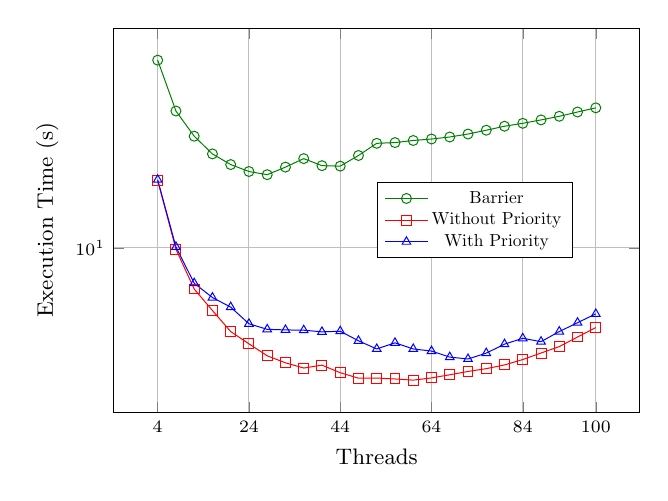
\begin{tikzpicture}[scale=0.9, transform shape]
        \begin{axis}[
            xlabel={Threads},
            ylabel={Execution Time (s)},
            % Using your paper's defined style
            myAxisStyle/.style={
                tick label style={font=\scriptsize},
                label style={font=\small},
                title style={at={(0.5,1.1)}, anchor=south, font=\small},
                grid=both,
                width=9cm, % Adjusted for slide width
                height=7cm
            },
            myAxisStyle,
            ymode=log,
            log basis y=10,
            xtick={4, 24, 44, 64, 84, 100},
            ytick={10, 100, 1000, 10000, 100000},
            legend style={at={(axis description cs:0.5,0.5)}, anchor=west, nodes={scale=0.7, transform shape}}
            ]
            % Barrier Data (Full dataset)
            \addplot[darkgreen, mark=o] coordinates {
                (4,60.32933) (8,37.08767) (12,29.13767) (16,24.59833)
                (20,22.211) (24,20.787) (28,20.160) (32,21.67867)
                (36,23.511) (40,21.980) (44,21.87833) (48,24.22767)
                (52,27.220) (56,27.414) (60,27.967) (64,28.367)
                (68,28.91533) (72,29.754) (76,30.85733) (80,32.056)
                (84,32.97067) (88,34.05467) (92,35.255) (96,36.73167)
                (100,38.23033)
            };
            \addlegendentry{Barrier};
            
            % Without Priority Data (Full dataset)
            \addplot[red, mark=square] coordinates {
                (4,19.068) (8,9.88267) (12,6.753) (16,5.495)
                (20,4.492) (24,3.996) (28,3.563) (32,3.33167)
                (36,3.169) (40,3.258) (44,3.030) (48,2.87633)
                (52,2.87967) (56,2.85433) (60,2.82233) (64,2.883)
                (68,2.971) (72,3.06733) (76,3.15033) (80,3.26467)
                (84,3.438) (88,3.65933) (92,3.891) (96,4.26467)
                (100,4.668)
            };
            \addlegendentry{Without Priority};
            
            % With Priority Data (Full dataset)
            \addplot[blue, mark=triangle] coordinates {
                (4,19.20933) (8,10.104) (12,7.13767) (16,6.22233)
                (20,5.67667) (24,4.84067) (28,4.59033) (32,4.56433)
                (36,4.55167) (40,4.48067) (44,4.507) (48,4.11267)
                (52,3.804) (56,4.03433) (60,3.80433) (64,3.72833)
                (68,3.518) (72,3.45633) (76,3.65533) (80,3.98367)
                (84,4.212) (88,4.07933) (92,4.493) (96,4.891)
                (100,5.32067)
            };
            \addlegendentry{With Priority};
        \end{axis}
      \end{tikzpicture}
    \end{figure}

    % ----- RIGHT: Concise text block for analysis -----
    \column{0.4\textwidth}
    \begin{block}{The Experiment}
      We measure execution time on a fixed-size matrix ($8192 \times 8192$) while increasing the number of threads.
    \end{block}
    
    \pause
    \begin{alertblock}{Key Findings}
      \begin{itemize}
        \item Our two-queue schedulers show strong scaling, with performance improving significantly as threads are added.
        \item The barrier-based method scales poorly due to synchronization overhead, becoming slower after an initial improvement.
      \end{itemize}
    \end{alertblock}

  \end{columns}
\end{frame}
	% Slide: End-to-End Impact on SLSQP (Corrected Layout)
\begin{frame}{Results: End-to-End Impact on SLSQP}

  \begin{columns}[c,onlytextwidth] % Vertically centered

    % ----- LEFT: The SLSQP performance graph -----
    \pause
    \column{0.6\textwidth}
    \begin{figure}
      \centering
      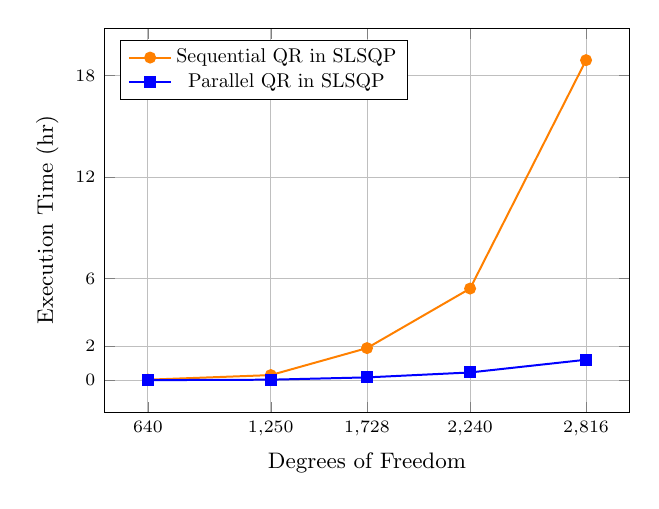
\begin{tikzpicture}[scale=0.9, transform shape]
        \begin{axis}[
            xlabel={Degrees of Freedom},
            ylabel={Execution Time (hr)},
            myAxisStyle/.style={
                tick label style={font=\scriptsize},
                label style={font=\small},
                grid=both,
                width=9cm,
                height=7cm
            },
            myAxisStyle,
            legend style={nodes={scale=0.8, transform shape}},
            xtick={640,1250,1728,2240,2816},
            ytick={0,2,6,12,18},
            legend pos=north west
            ]
            \addplot[orange, mark=*, thick] coordinates { (640,0.02908) (1250,0.3004) (1728,1.89514) (2240,5.415) (2816,18.91215) };
            \addlegendentry{Sequential QR in SLSQP};
            \addplot[blue, mark=square*, thick] coordinates { (640,0.001454) (1250,0.02879) (1728,0.16458) (2240,0.456) (2816,1.20716) };
            \addlegendentry{Parallel QR in SLSQP};
        \end{axis}
      \end{tikzpicture}
    \end{figure}

    % ----- RIGHT: Concise bullet points for context and results -----
    \column{0.4\textwidth}
    \begin{block}{Context}
      \begin{itemize}
        \item We integrated our parallel QR into the full SLSQP solver.
        \item \textbf{DOF (Degrees of Freedom):} Total problem variables. More DOF = larger matrix.
      \end{itemize}
    \end{block}
    
    \pause
    \begin{alertblock}{Final Result}
      At 2,816 DOF:
      \begin{itemize}
        \item Sequential: \textbf{18.9 hours}
        \item Parallel: \textbf{1.2 hours}
        \item \textbf{> 15x Speedup}
      \end{itemize}
    \end{alertblock}

  \end{columns}
\end{frame}
	% Final Slide: Comparison with PLASMA (with Corrected Graph)
\begin{frame}{SOTA - Plasma Comparison}

	\begin{columns}[c,onlytextwidth]
	
		% ----- LEFT: The comparison graph with your data -----
		\column{0.30\textwidth}
		% PGFPlots code for the PLASMA comparison graph (128-4096)
		
		\pause
		\begin{figure}
			\centering
			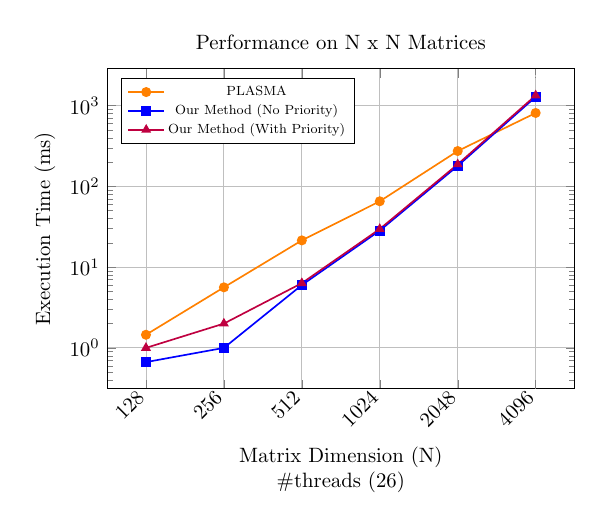
\begin{tikzpicture}[scale=0.75, transform shape]
				\begin{axis}[
				title={Performance on N x N Matrices},
					xlabel={%
					\begin{tabular}{c} % Use a tabular environment for multi-line text
					Matrix Dimension (N) \\
					\#threads (26)
					\end{tabular}%
					},
					ylabel={Execution Time (ms)},
					ymode=log,
					xmode=normal,
					log basis y=10,
					symbolic x coords={128, 256, 512, 1024, 2048, 4096},
					xtick=data,
					xticklabel style={rotate=45, anchor=east},
					grid=major,
					width=9.5cm, % Reduced width to prevent overflow
					height=7cm,
					extra x ticks={4096},
					extra x tick labels={},
					extra x tick style={grid=major, dashed, depred}, % Comma is here
					legend style={
					font=\footnotesize,
					at={(0.03,0.97)},
					anchor=north west,
					nodes={scale=0.8, transform shape}
					}
					]
					
					\addplot[orange, mark=*, thick] coordinates { (128, 1.454) (256, 5.62) (512, 21.434) (1024, 65.37) (2048, 273.851) (4096, 810.618) };
					\addlegendentry{PLASMA};
					\addplot[blue, mark=square*, thick] coordinates { (128, 0.6667) (256, 1.0) (512, 6.0) (1024, 28.3333) (2048, 179.3333) (4096, 1283.3333) };
					\addlegendentry{Our Method (No Priority)};
					\addplot[purple, mark=triangle*, thick] coordinates { (128, 1.0) (256, 2.0) (512, 6.3333) (1024, 29.6667) (2048, 187.6667) (4096, 1335.6667) };
					\addlegendentry{Our Method (With Priority)};					
				\end{axis}
			\end{tikzpicture}
		\end{figure}
		
		% ----- RIGHT: The narrative and analysis -----
		\pause
		\column{0.5\textwidth}
		\begin{block}{Key Takeaways}
		  \begin{itemize}
			 \item Our approach achieves a \textbf{2--3$\times$ speedup} over PLASMA (current SOTA)
			       for sizes 128$\times$128 to 2048$\times$2048.  
			 \item Relies only on \textbf{regular compiler optimizations} and our scheduling logic.  
			 \item PLASMA depends on \textbf{BLAS routines}, which are hand-optimized using intrinsics.  
			 \item Performance drops for $>$2048, but the relevant range (up to 2048) 
			  directly matches \textbf{structural engineering and non-linear programming workloads}, 
			  where solver speed is a critical bottleneck.	
		  \end{itemize}
		\end{block}
	
	\end{columns}
\end{frame}

	% Slide: Related Work
\begin{frame}{Related Work \& Our Contribution}

	\begin{columns}[T,onlytextwidth]	
		\pause 
		\column{0.45\textwidth}
		\begin{block}{Advances in Optimization Solvers}
		  \begin{itemize}
		    \item Solvers like \textbf{IPOPT} and \textbf{SNOPT} are continuously evolving.
		    \item NLOPT's \textbf{SLSQP}, while popular, has lacked recent performance updates.
		    \item \textbf{PySLSQP} improved usability, but not core computational speed.
		  \end{itemize}
		\end{block}
		
		% ----- RIGHT: Existing Work in Parallel QR -----
		\column{0.5\textwidth}
		\begin{block}{Advances in Parallel QR Factorization}
		  \begin{itemize}
		    \item Significant research exists on parallelizing QR, often using task-based DAG scheduling.
		    \item Key works (Buttari et al., Baskaran et al.) have explored tiled methods and dynamic scheduling with priority queues.
		  \end{itemize}
		\end{block}	
	\end{columns}

	\pause 
\begin{alertblock}{The Gap \& Our Contribution}
    \begin{itemize}
      \item \textbf{The Challenge:} Achieving low-overhead, high-performance QR factorization for the \textbf{small-to-medium matrix sizes} common in iterative solvers.
      \item \textbf{Our Contribution:} Our lightweight scheduler is specifically designed for this scenario, delivering a \textbf{2-3x speedup} over mature libraries in this critical range.
    \end{itemize}
  \end{alertblock}

\end{frame}
	% Slide: Conclusion & Future Work
\begin{frame}{Conclusion}

  \begin{columns}[c,onlytextwidth]
		% ----- LEFT: What We Achieved -----
		\pause
		\column{0.43\textwidth}
		\begin{block}{What We Achieved}
		  \begin{itemize}
		    \item Modeled the sequential QR algorithm as a task-based DAG to expose parallelism.
		    \item Designed a novel, asynchronous two-queue scheduler to execute the DAG without barriers.
		    \item Integrated our high-performance parallel QR into the NLOPT SLSQP solver.
		    \item Demonstrated a \textbf{>15x end-to-end speedup} on large-scale problems.
		  \end{itemize}
		\end{block}
		
		\pause
		\column{0.50\textwidth}
  \begin{alertblock}{Overall Impact}
    \centering
    Our work delivers a lightweight, open-source scheduler that significantly accelerates SLSQP for the common, medium-sized workloads where performance is most critical.
  \end{alertblock}
    \end{columns}

\end{frame}
	% Slide: Thank You & Questions
\begin{frame}{Thank You}
  
  \vspace*{\fill} % Pushes the content to the vertical center of the slide
  
  \begin{columns}[T,onlytextwidth]
    
    % ----- LEFT: Main message and contact info -----
    \column{0.6\textwidth}
    \centering
    \Huge \textbf{Questions?}
    
    \vspace{1.5cm}
    
  
    
    \normalsize
    Team: \\
    \small
    Soumyajit Chatterjee, Rahul Utkoor, Uppu Eshwar, \\ Sathya Peri, V.K. Nandivada
    
    % ----- RIGHT: The artifact QR code -----
    \column{0.4\textwidth}
    \begin{block}{Artifact}
      \centering
      % NOTE: The link is from your paper's Zenodo reference.
      \qrcode[height=4cm]{https://doi.org/10.5281/zenodo.15602262}
      
      \vspace{2mm}
      \href{https://github.com/PDCRL/ParSQP}{github.com/PDCRL/ParSQP}
    \end{block}
    
  \end{columns}
  
  \vspace*{\fill} % Balances the vertical centering
  
\end{frame}

\end{document}


    